% sections/chapter1.tex
\chapter{Introduction}
\label{sec:introduction}

This chapter provides a comprehensive overview of the CORAL project's Iteration 1, establishing the foundation for our multi-hypothesis ASR correction architecture. We present the problem domain, articulate the specific research challenges, and outline the objectives achieved during this initial development phase.

\section{Problem Domain}

Automatic Speech Recognition (ASR) systems have achieved remarkable success in high-resource languages such as English and Mandarin. However, low-resource languages like Urdu continue to face significant performance challenges. Urdu, spoken by over 230 million people worldwide, presents unique difficulties for ASR systems due to:

\begin{itemize}
    \item \textbf{Limited Training Data}: Scarcity of large-scale, high-quality annotated speech datasets compared to high-resource languages.
    \item \textbf{Linguistic Complexity}: Rich morphological structure, extensive use of diacritics, and complex phonetic patterns.
    \item \textbf{Code-Switching}: Frequent mixing with English and regional languages in conversational speech.
    \item \textbf{Dialectal Variation}: Multiple regional dialects with distinct acoustic and linguistic characteristics.
    \item \textbf{Script Ambiguity}: Perso-Arabic script with optional diacritical marks leads to ambiguous representations.
\end{itemize}

Current state-of-the-art pre-trained ASR models for Urdu, including fine-tuned variants of Whisper, Wav2Vec2-XLSR, and other multilingual models, still exhibit Word Error Rates (WER) exceeding 35\% on standard benchmarks. This performance ceiling significantly limits the practical deployment of ASR systems in critical domains such as healthcare, education, legal documentation, and accessibility technologies for the Urdu-speaking population.

\subsection{Current Limitations of Single-Model ASR Systems}

Single-model ASR architectures suffer from three fundamental limitations:

\begin{enumerate}
    \item \textbf{Deterministic Predictions}: Models produce a single best hypothesis without considering alternative interpretations, even when multiple plausible transcriptions exist.
    \item \textbf{Lack of Uncertainty Quantification}: No explicit mechanism to indicate confidence in predictions, making it difficult to identify and correct errors.
    \item \textbf{Domain Brittleness}: Models trained or fine-tuned on specific domains fail to generalize to out-of-domain audio, code-switched speech, or dialectal variations.
\end{enumerate}

\section{Research Problem Statement}

The CORAL project addresses the following research problem:

\textit{Current state-of-the-art pre-trained ASR models for Urdu exhibit Word Error Rates exceeding 35\% on standard benchmarks and suffer significant performance degradation on out-of-domain and code-switched speech. Single-model systems make deterministic predictions without considering alternative interpretations or providing uncertainty estimates. When the model's top prediction is incorrect, there is no mechanism for recovery or correction.}

This leads to three critical challenges:

\begin{enumerate}
    \item \textbf{Ambiguity Mismanagement}: For phonetically similar Urdu words or in noisy audio conditions, a single model's highest-probability output may be incorrect, with no indication of uncertainty.
    \item \textbf{Lack of Robustness}: Individual models cannot effectively generalize to the diverse domains, dialects, and code-switching patterns characteristic of real-world Urdu speech.
    \item \textbf{Error Propagation}: Errors made by ASR models propagate to downstream applications (translation, summarization, information retrieval) without any correction mechanism.
\end{enumerate}

\subsection{Research Hypothesis}

Our hypothesis states: \textit{By leveraging word-level confidence scores from an ensemble of diverse pre-trained ASR models and using a black-box instruction-tuned Large Language Model (LLM) to intelligently synthesize these confidence-annotated hypotheses, we can create a system that produces final transcripts with significantly lower WER than any individual model, thereby establishing a new state-of-the-art for Urdu ASR without requiring model fine-tuning.}

\section{Proposed Solution: The CORAL Framework}

CORAL (Consensus-based Refinement And Learning) is a novel two-stage "Generate-and-Refine" architecture that combines the strengths of multiple ASR models with the reasoning capabilities of instruction-tuned LLMs.

\subsection{Architecture Overview}

The CORAL framework consists of two main stages:

\begin{enumerate}
    \item \textbf{Stage 1: Multi-Model Hypothesis Generation with Confidence Extraction}
    \begin{itemize}
        \item Deploy an ensemble of diverse pre-trained ASR models
        \item Extract word-level confidence scores from each model's output
        \item Generate multiple confidence-annotated hypotheses for each audio input
    \end{itemize}
    
    \item \textbf{Stage 2: Instruction-Guided Hypothesis Correction} (To be implemented in Iteration 2)
    \begin{itemize}
        \item Feed all hypotheses with confidence annotations to a black-box LLM
        \item Use structured prompts to guide intelligent synthesis
        \item Generate final transcript by leveraging confidence scores and linguistic coherence
    \end{itemize}
\end{enumerate}

\begin{figure}[htbp]
    \centering
    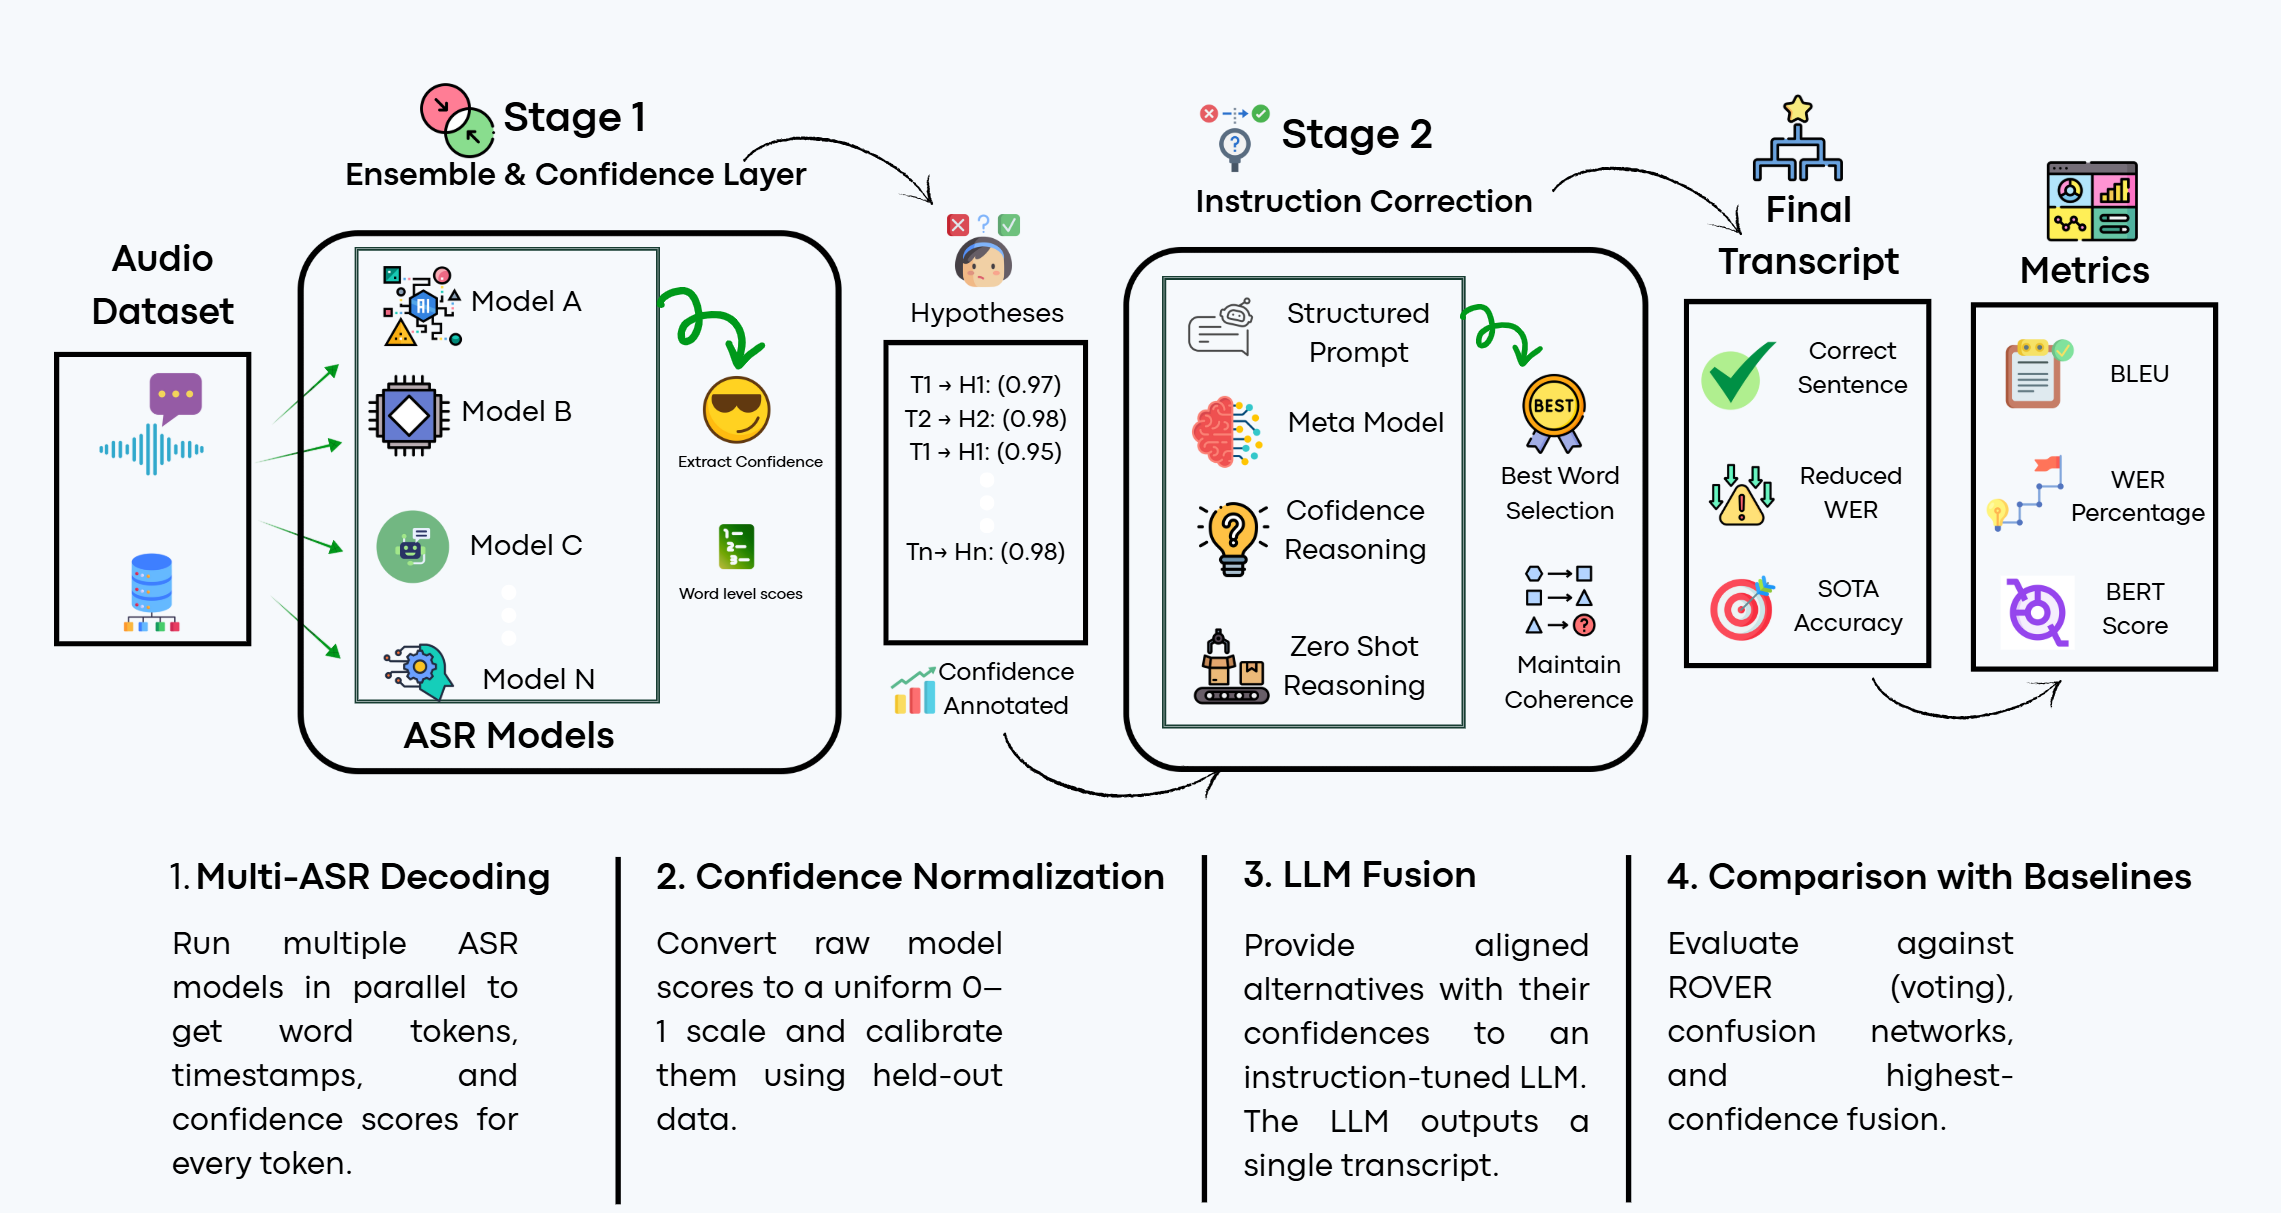
\includegraphics[width=0.95\textwidth]{ThesisFigs/coral-white.png}
    \caption{CORAL Architecture: Two-stage pipeline with Multi-Model Hypothesis Generation and Instruction-Guided Correction}
    \label{fig:coral_architecture}
\end{figure}

\subsection{Stage 1: Multi-Model Hypothesis Generation (Iteration 1 Focus)}

Iteration 1 focuses exclusively on implementing Stage 1. We employ four distinct ASR models, each providing complementary strengths:

\begin{itemize}
    \item \textbf{Whisper (Multiple Variants)}: OpenAI's multilingual encoder-decoder model with robust cross-domain performance
    \begin{itemize}
        \item Whisper Large (v3): 1.5B parameters, highest accuracy
        \item Whisper Medium: 769M parameters, balanced performance
        \item Whisper Small: 244M parameters, efficiency-optimized
    \end{itemize}
    
    \item \textbf{Wav2Vec2-XLSR}: Facebook's cross-lingual speech representation model fine-tuned specifically for Urdu
    \begin{itemize}
        \item 300M parameters
        \item Self-supervised pre-training on multilingual speech
        \item Specialized Urdu fine-tuning
    \end{itemize}
\end{itemize}

\subsection{Confidence Score Extraction Methodology}

For each model architecture, we implement specific confidence extraction techniques:

\begin{enumerate}
    \item \textbf{Encoder-Decoder Models (Whisper)}:
    \begin{itemize}
        \item Extract token log-probabilities using \texttt{output\_scores=True} in HuggingFace's \texttt{generate()} method
        \item Apply softmax to scores for probability normalization
        \item Average token probabilities for word-level confidence
    \end{itemize}
    
    \item \textbf{CTC Models (Wav2Vec2)}:
    \begin{itemize}
        \item Extract output logits from final CTC layer
        \item Apply softmax to obtain token probability distributions
        \item Use maximum probability across frames as token confidence
        \item Aggregate for word-level scores
    \end{itemize}
\end{enumerate}

\section{Iteration 1 Objectives and Scope}

The primary objectives of Iteration 1 (September - October 2025) were:

\begin{enumerate}
    \item \textbf{Infrastructure Development}: Integrate ensemble of pre-trained ASR models, implement audio preprocessing pipeline, and develop model loading and memory management system.
    \item \textbf{Confidence Extraction Implementation}: Implement word-level confidence score extraction for each model type, validate confidence calibration metrics, and ensure consistent output format across all models.
    \item \textbf{Baseline Evaluation}: Establish baseline WER, CER, and confidence metrics for each model, analyze confidence calibration using Expected Calibration Error (ECE), and identify best-performing individual model.
    \item \textbf{Web Interface Development}: Create real-time audio recording and upload interface, implement live transcription with word-level confidence visualization, and build dataset collection and management system.
\end{enumerate}

\subsection{Deliverables}

Iteration 1 produced the following deliverables:

\begin{itemize}
    \item \textbf{Working Pipeline}: Complete implementation of Stage 1 producing confidence-annotated hypotheses from all models
    \item \textbf{Web Application}: Flask-based interface with real-time recording, transcription, and dataset collection
    \item \textbf{Evaluation Framework}: Comprehensive metrics computation including WER, CER, confidence scores, and ECE
    \item \textbf{Baseline Results}: Performance benchmarks for all four models on test dataset
    \item \textbf{Documentation}: Complete codebase with inline documentation and usage examples
\end{itemize}

\section{Report Organization}

The remainder of this report is organized as follows: Chapter 2 presents a comprehensive literature review analyzing related work in multi-ASR fusion, confidence estimation, LLM-based correction, and low-resource ASR. Chapter 3 details the implementation, experimental setup, evaluation metrics, and baseline results from Iteration 1.

\section{Summary}

Iteration 1 successfully established the foundational infrastructure for the CORAL system. We have implemented a robust multi-model ASR pipeline with confidence extraction capabilities, created an evaluation framework, and established baseline performance metrics. The system is now ready for the integration of the instruction-guided correction mechanism in Iteration 2, which will leverage the confidence-annotated hypotheses generated in this iteration to produce improved final transcripts.